\section{Fa struktúra ábrázolása}
	Amikor először találkoztam az Oracle online vizualizációs eszközével, és felmértem a lehetőségeit, a legelső ami feltűnt nekem, hogy választható megjelenések között szerepel több fa struktúra megjelenítésére alkalmas eszköz. Ebben a fejezetben egy ilyen fa struktúrát fogok megjeleníteni.
	
	\subsection{Adathalmaz}
	A fa struktúrát képező szerkezetek mind megjelenítése, mind tárolása komoly feladat egy fejlesztési ciklusban. A megjelenítés rekurzív vagy iteratív látásmódot igényel, hiszen egy fa struktúra mélységéről sosincs információnk, elméletben akármilyen mély lehet. A tárolás szempontjából pedig pont azért nehézkes, mert a struktúrára vonatkozó információkat kell elfednünk, hiszen legtöbbször ezek az adatok sima relációs adatbázisokban vannak letárolva. A feladat bemutatására egy a valóságból hozott példán (szerkezet) keresztül szeretném megvizsgálni, hogy az eszköz képes-e ennek a struktúrának a megjelenítésére. Ehhez az adatokat generáltattam, de struktúrát korábbi ismereteimből hoztam. Ehhez az egyszerűsített menüszerkezethez három oszlopra van csak szükségünk, \textit{id}, \textit{parent\_id}, \textit{name}. Az \textit{id} az egyedi azonosító (inkrementális egész szám). A \textit{parent\_id} egy \textit{id}-re való hivatkozás, hogy az adott elem melyik elem alá tartozik. Ez a mező tartalmazza a strukturális információt. A főmenük \textit{parent\_id}-ja 0. Végezetül egy \textit{name}, ami az adott menüpont neve. A vizsgálathoz 100 adatot generáltam. Az adat tábla tartalmát a \ref{fig:pokedata}. ábra mutatja be.
	
	\begin{figure}[h!]
		\centering
		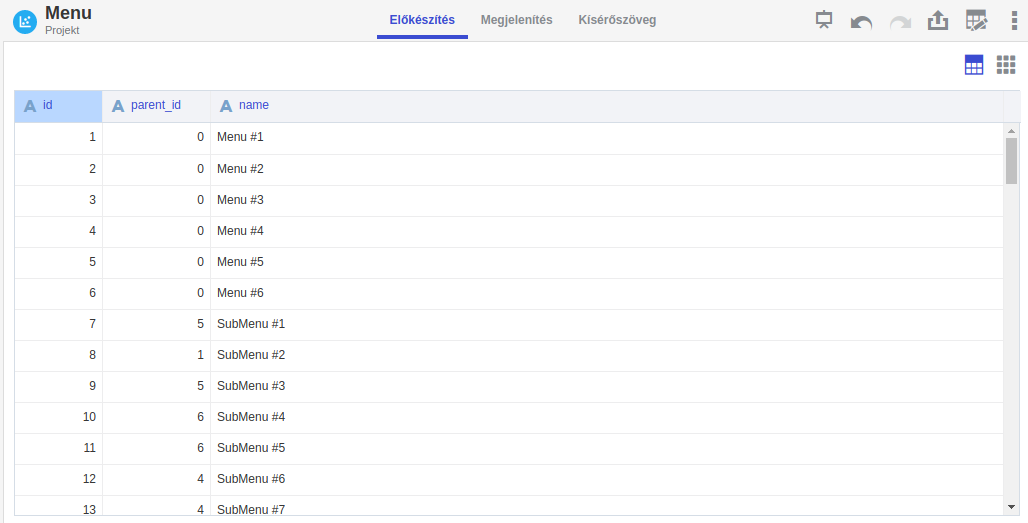
\includegraphics[width=1.0\linewidth]{keve_imgs/adat}
		\caption{Fa struktúrához felhasznált adatok}
		\label{fig:faadat}
	\end{figure}
	
	Az ábrából jól látszik, hogy a struktúrára nagyon nehezen tudunk csak következtetni egy táblázatból, még akkor is, ha most esetünkben éppen kedvező sorrendben vannak az egyes elemek.

	\subsection{Megjelenések}
	Az alfejezet címe mád mutatja, hogy több sikeres megoldás is született, így most ezeken fogok végigmenni.
	
		\subsubsection{Ajánlott}
		Az eszköz felajánl egy szerinte legjobbnak vélt megjelenítést. Ez esetünkben sajnos nem járt sikerrel, mivel minden áron táblázatba akarta megjeleníteni az adatokat úgy is, hogy nem volt mérőszám típusú oszlop. Az ajánlott legjobb megjelenítést a \ref{fig:legjobbmegjelenites}. ábra mutatja be. Ezen a téren még van mit fejlődni.
		
		\begin{figure}[h!]
			\centering
			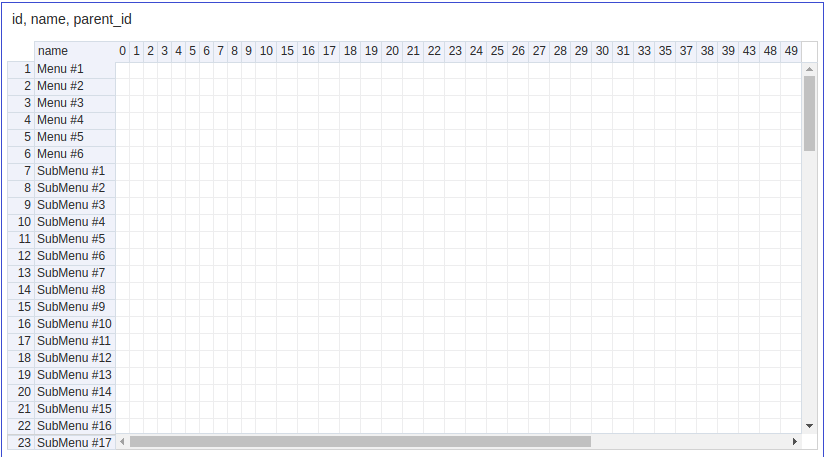
\includegraphics[width=1.0\linewidth]{keve_imgs/legjobbmegjelenites}
			\caption{Oracle által ajánlott legjobb megjelenítés}
			\label{fig:legjobbmegjelenites}
		\end{figure}
	
		\subsubsection{Fa}
		Az általam legjobbnak elképzelt megjelenítési struktúra. Habár sokadik próbálkozásra sem sikerült a végső pontokban az adott elem nevét megjeleníteni az id helyett, mégis a struktúrát jól képes megjeleníteni az eszköz. A fa megjelenítést a \ref{fig:famegjelenites}. ábra mutatja be. Az ábrán jól látszik a struktúra, minden egyes gyerek-szülő kapcsolat is nyomon követhető. Talán az elforgatás, és a név kiírásának hiánya rontott az összképen. Mindenesetre ez egy olyan információt képes megjeleníteni, amelyet az adatok ismeretében is nehéz fejben elképzelni.		
		
		\begin{figure}[h!]
			\centering
			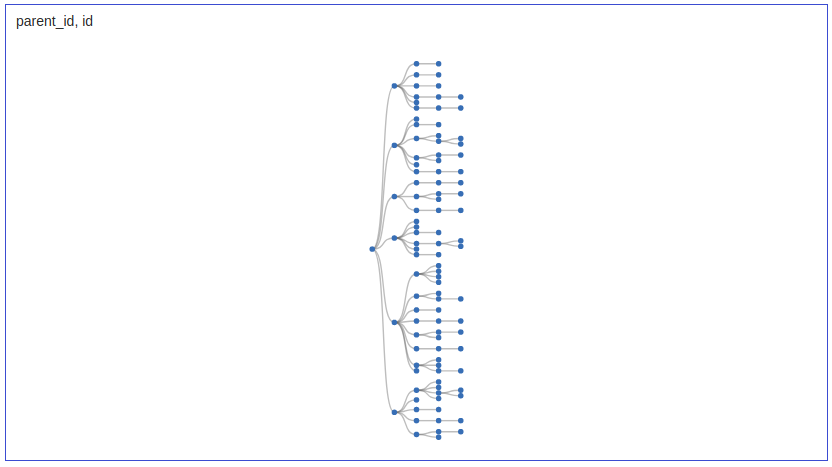
\includegraphics[width=1.0\linewidth]{keve_imgs/famegjelenites}
			\caption{Fa megjelenítés}
			\label{fig:famegjelenites}
		\end{figure}
	
		\subsubsection{Fatérkép}
		A fatérkép megjelenítést azért választottam, hogy bemutatom, mert ez volt az egyetlen nézet, amin sikerült elérnem azt, hogy az egyedi azonosítókon kívül az adott elem neve is megjelenjen. Ez nyilván az ember számára jobban olvasható, átlátható megjelenítést eredményez. Ebben a megjelenítésben a menüpontok nevei vannak összeszedve, és csoportosítva vannak a szülő egyedi azonosítói szerint. Sajnos itt nem teljesen sikerül átadni a strukturális információt, habár az elemek nagysága a gyerekeinek számától függ.. A fatérkép megjelenítést a \ref{fig:faterkepmegjelenites}. ábra mutatja be. A megjelenés picit félrevezető, hiszen generált adatokról van szó, és az összes nem főmenü elem neve \textit{Submenu \#n}.
		
		\pagebreak	

		\begin{figure}[h!]
			\centering
			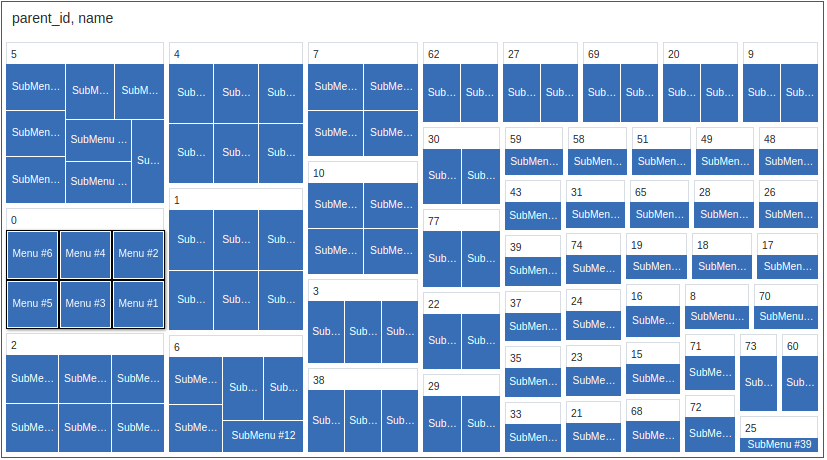
\includegraphics[width=1.0\linewidth]{keve_imgs/faterkepmegjelenites}
			\caption{Fatérkép megjelenítés}
			\label{fig:faterkepmegjelenites}
		\end{figure}
	
		\subsubsection{Sankey}
		A Sankey diagram eredetileg folyamatok ábrázolására lett tervezve, de az általam meghatározott feladat teljesítésére is alkalmas, sőt. Talán ez a megjelenítési mód tetszett a legjobban. Látványos, mégis sokat mond az adathalmazról. Az elkészült diagram a \ref{fig:sankeymegjelenites}. ábrán látható.	

		\begin{figure}[h!]
			\centering
			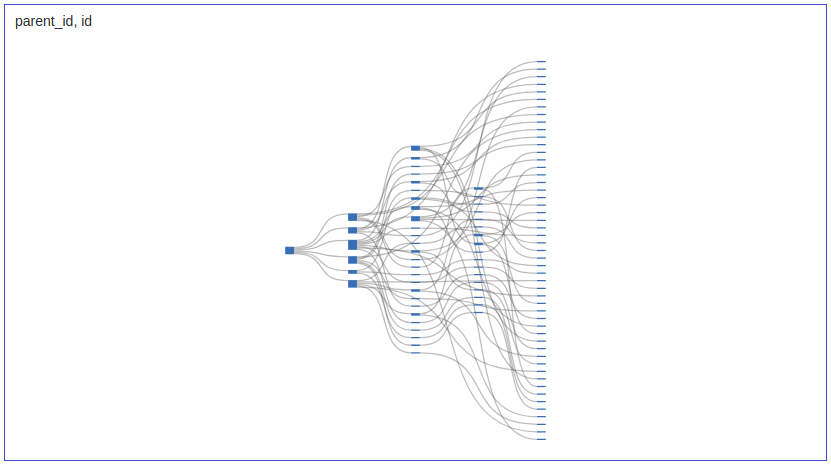
\includegraphics[width=1.0\linewidth]{keve_imgs/sankeymegjelenites}
			\caption{Sankey megjelenítés}
			\label{fig:sankeymegjelenites}
		\end{figure}	

		Az diagram két fontos tényezőjében tér el a fa diagramtól. Az egyik, hogy az adott csomópont nagyságával ránézésre látszik, hogy melyik elem tartalmazza a legtöbb gyerek elemet. Ez esztétikailag is jobban mutat, illetve segíti a könnyebb kiigazodást. Másrészt ennél a típusú diagramnál az utolsó gyerekek egy vonalban helyezkednek el. Így az utolsó oszlopban az összes (tényleges) végpont található. Jelen példánkban balról jobbra találhatóak a főmenük, almenük, al-almenük és a végpontok. Az ábrából például egyből látszik (ami a fán nem látszott), hogy a legkevesebb elem az al-almenükben van. Azonban további optikai plusz hatásra is képes az eszköz. A \ref{fig:sankeymegjelenites_reszlet}. ábra azt mutatja, ahogy egy kiválasztott csomópontra kattintva mi történik.
		
		\pagebreak	
		
		\begin{figure}[h!]
			\centering
			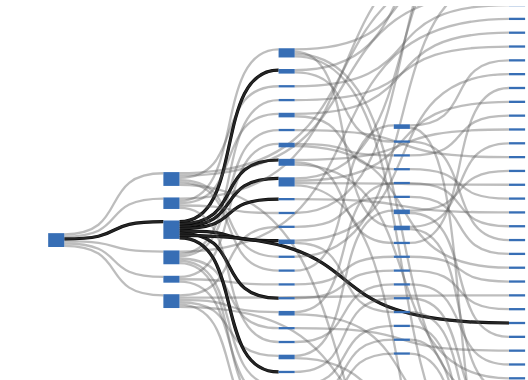
\includegraphics[width=1.0\linewidth]{keve_imgs/sankeymegjelenites_reszlet}
			\caption{Sankey megjelenítés részlet}
			\label{fig:sankeymegjelenites_reszlet}
		\end{figure}
		
		Ahogy az látható, azok az útvonalak, amelyekben az adott elem érintett, elszíneződnek. Az elszíneződésből látszik, hogy, habár a választási lehetőséget nagy része további menübe visz át minket, mégis van olyan amelyik például egyből végpontba visz.
	